\section{Ensamblado de la placa final}
    Al terminar el diseño del PCB, se consultaron con proveedores nacionales para la impresión de la placa. Ante la falta de respuesta, se optó por un proveedor internacional, PCBWay \cite{pcbway}. Todo el proceso, desde el envío de los archivos gerber, revisión y cambios, hasta recibir el paquete, llevó aproximadamente 15 días. Las placas recibidas son las que muestra la figura \ref{fig:placassolas}.
\begin{figure}
    \centering
    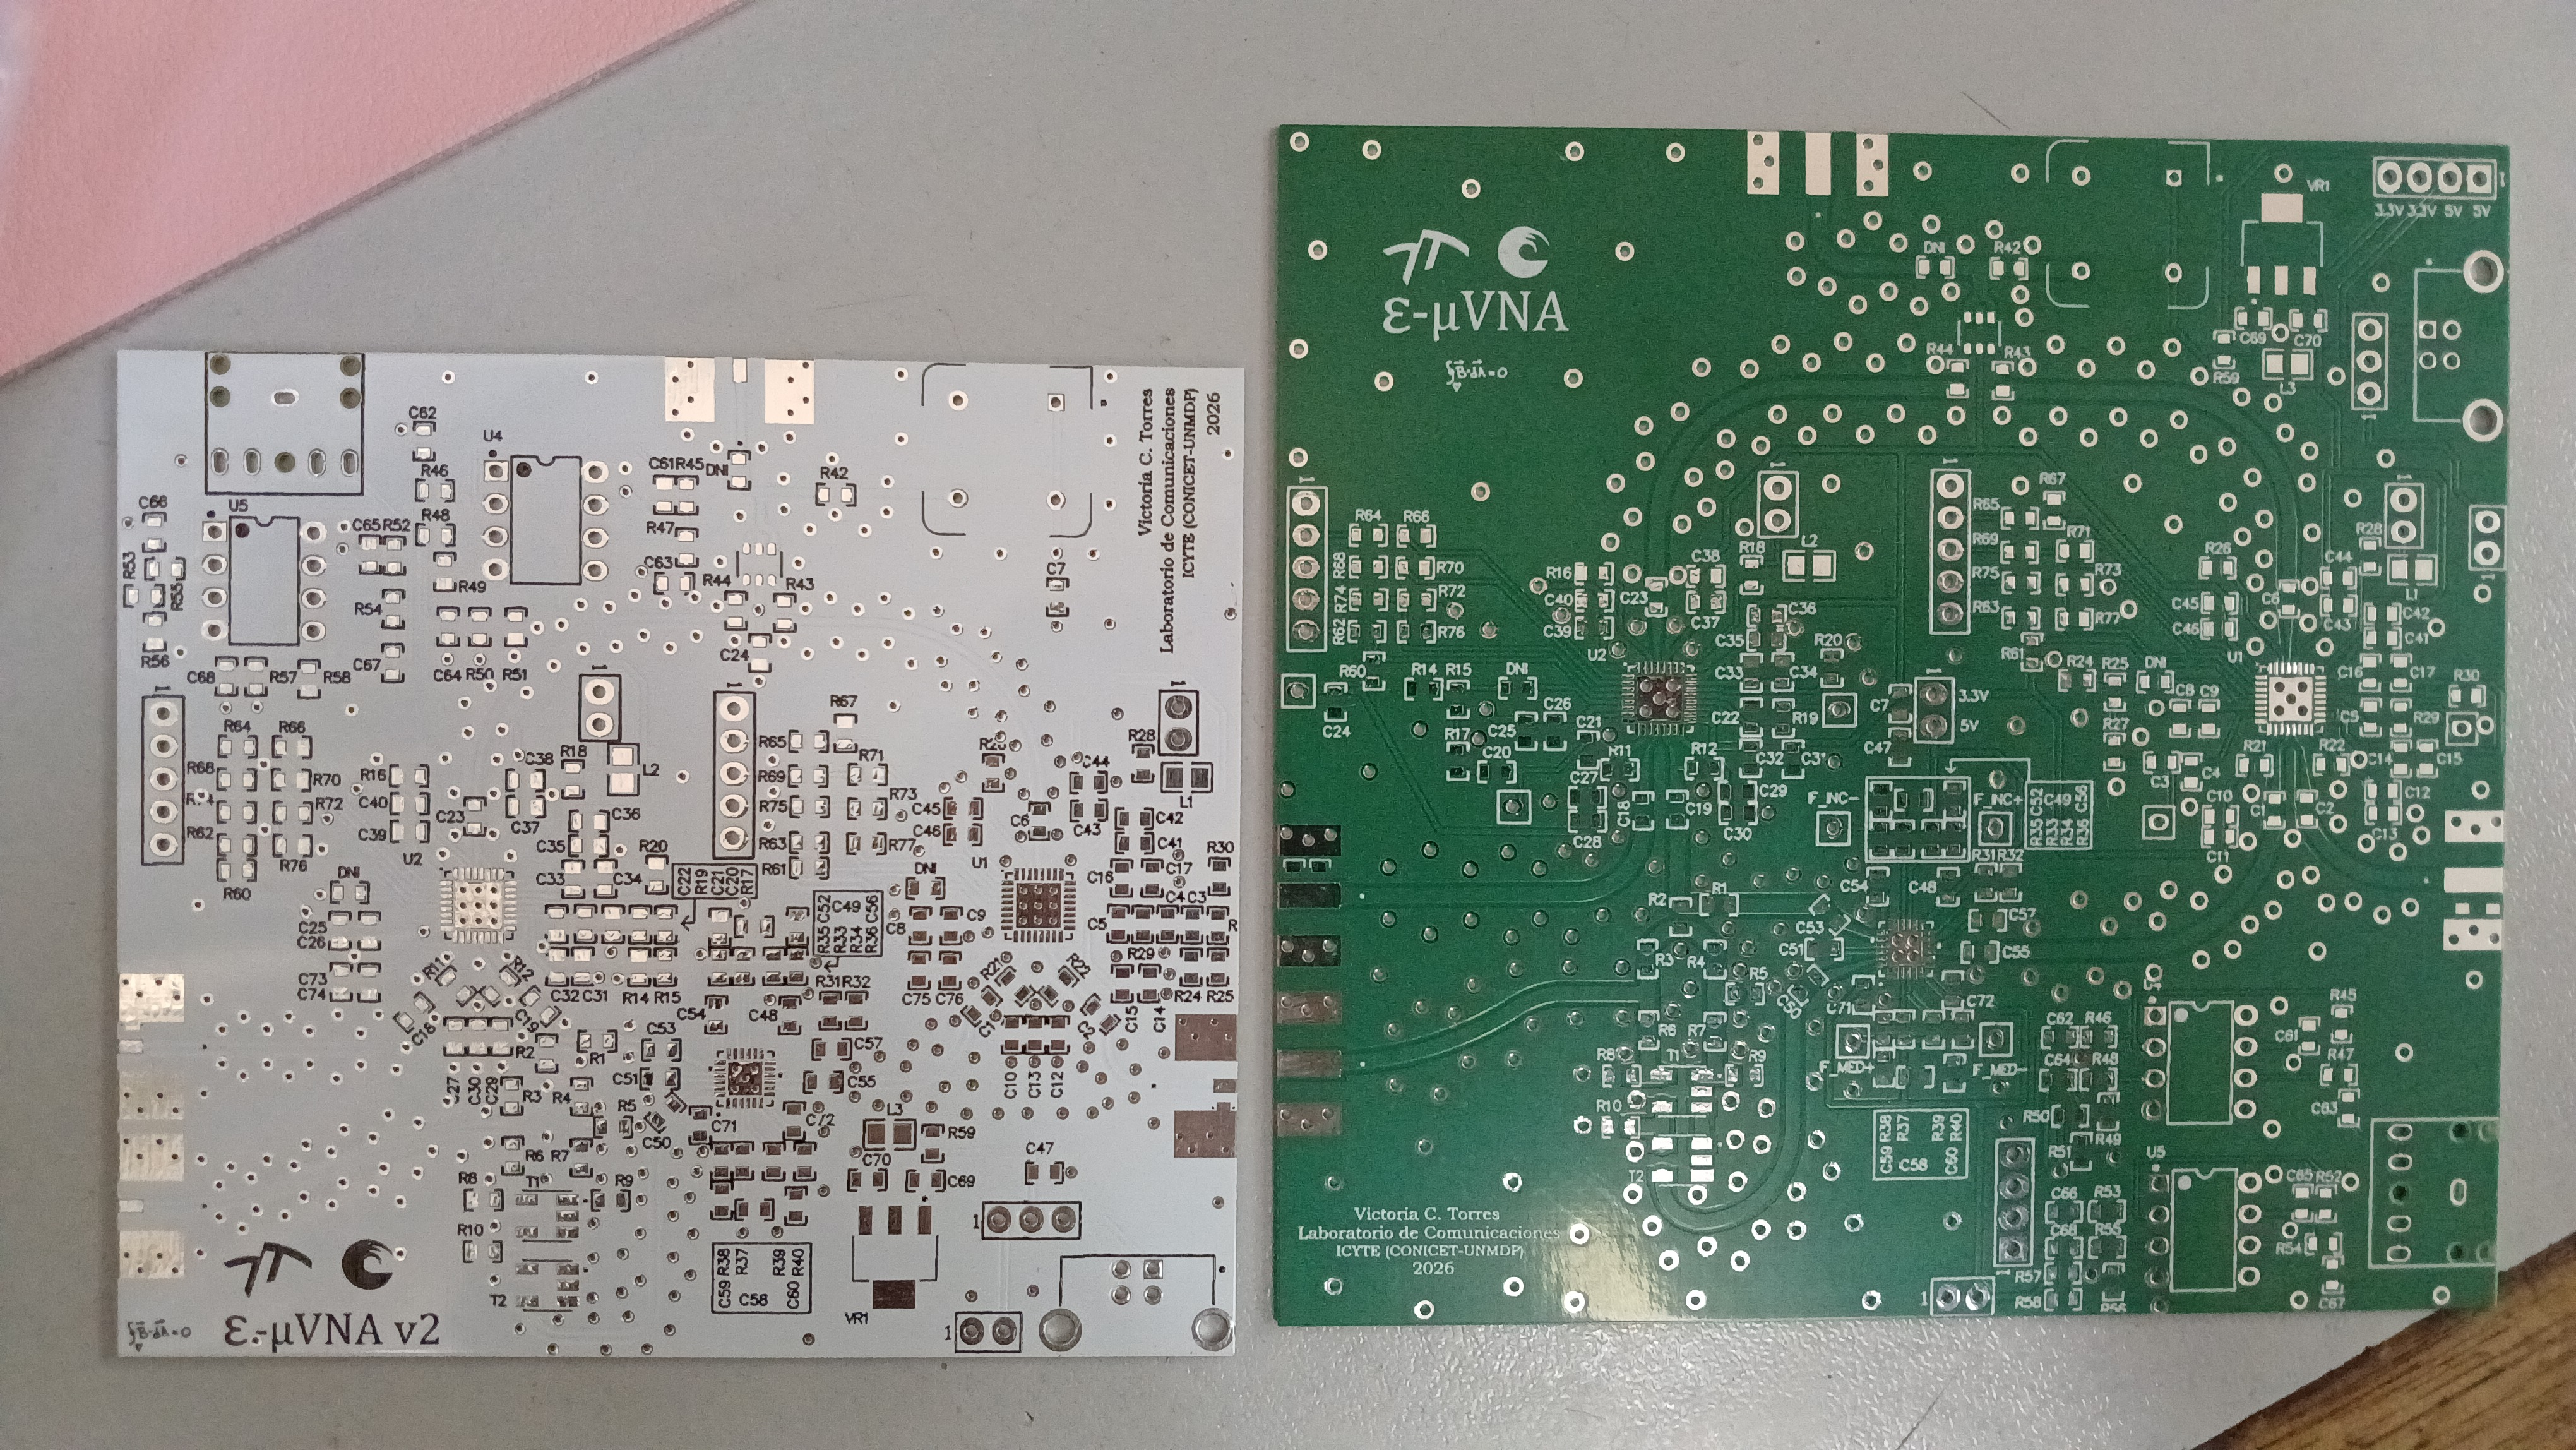
\includegraphics[width=0.8\linewidth]{Imagenes/placassolas.jpeg}
    \caption{Placas sin soldar}
    \label{fig:placassolas}
\end{figure}

    Los componentes se soldaron a mano, siendo los primeros  los tipo QFN (encapsulados planos cuádruples sin terminales - \textit{Quad Flat No-Lead}). Se puede observar en la figura \ref{fig:qfn} que para hacerlo se utilizó una estación de precalentamiento y un soldador de aire. 
\begin{figure}
    \centering
    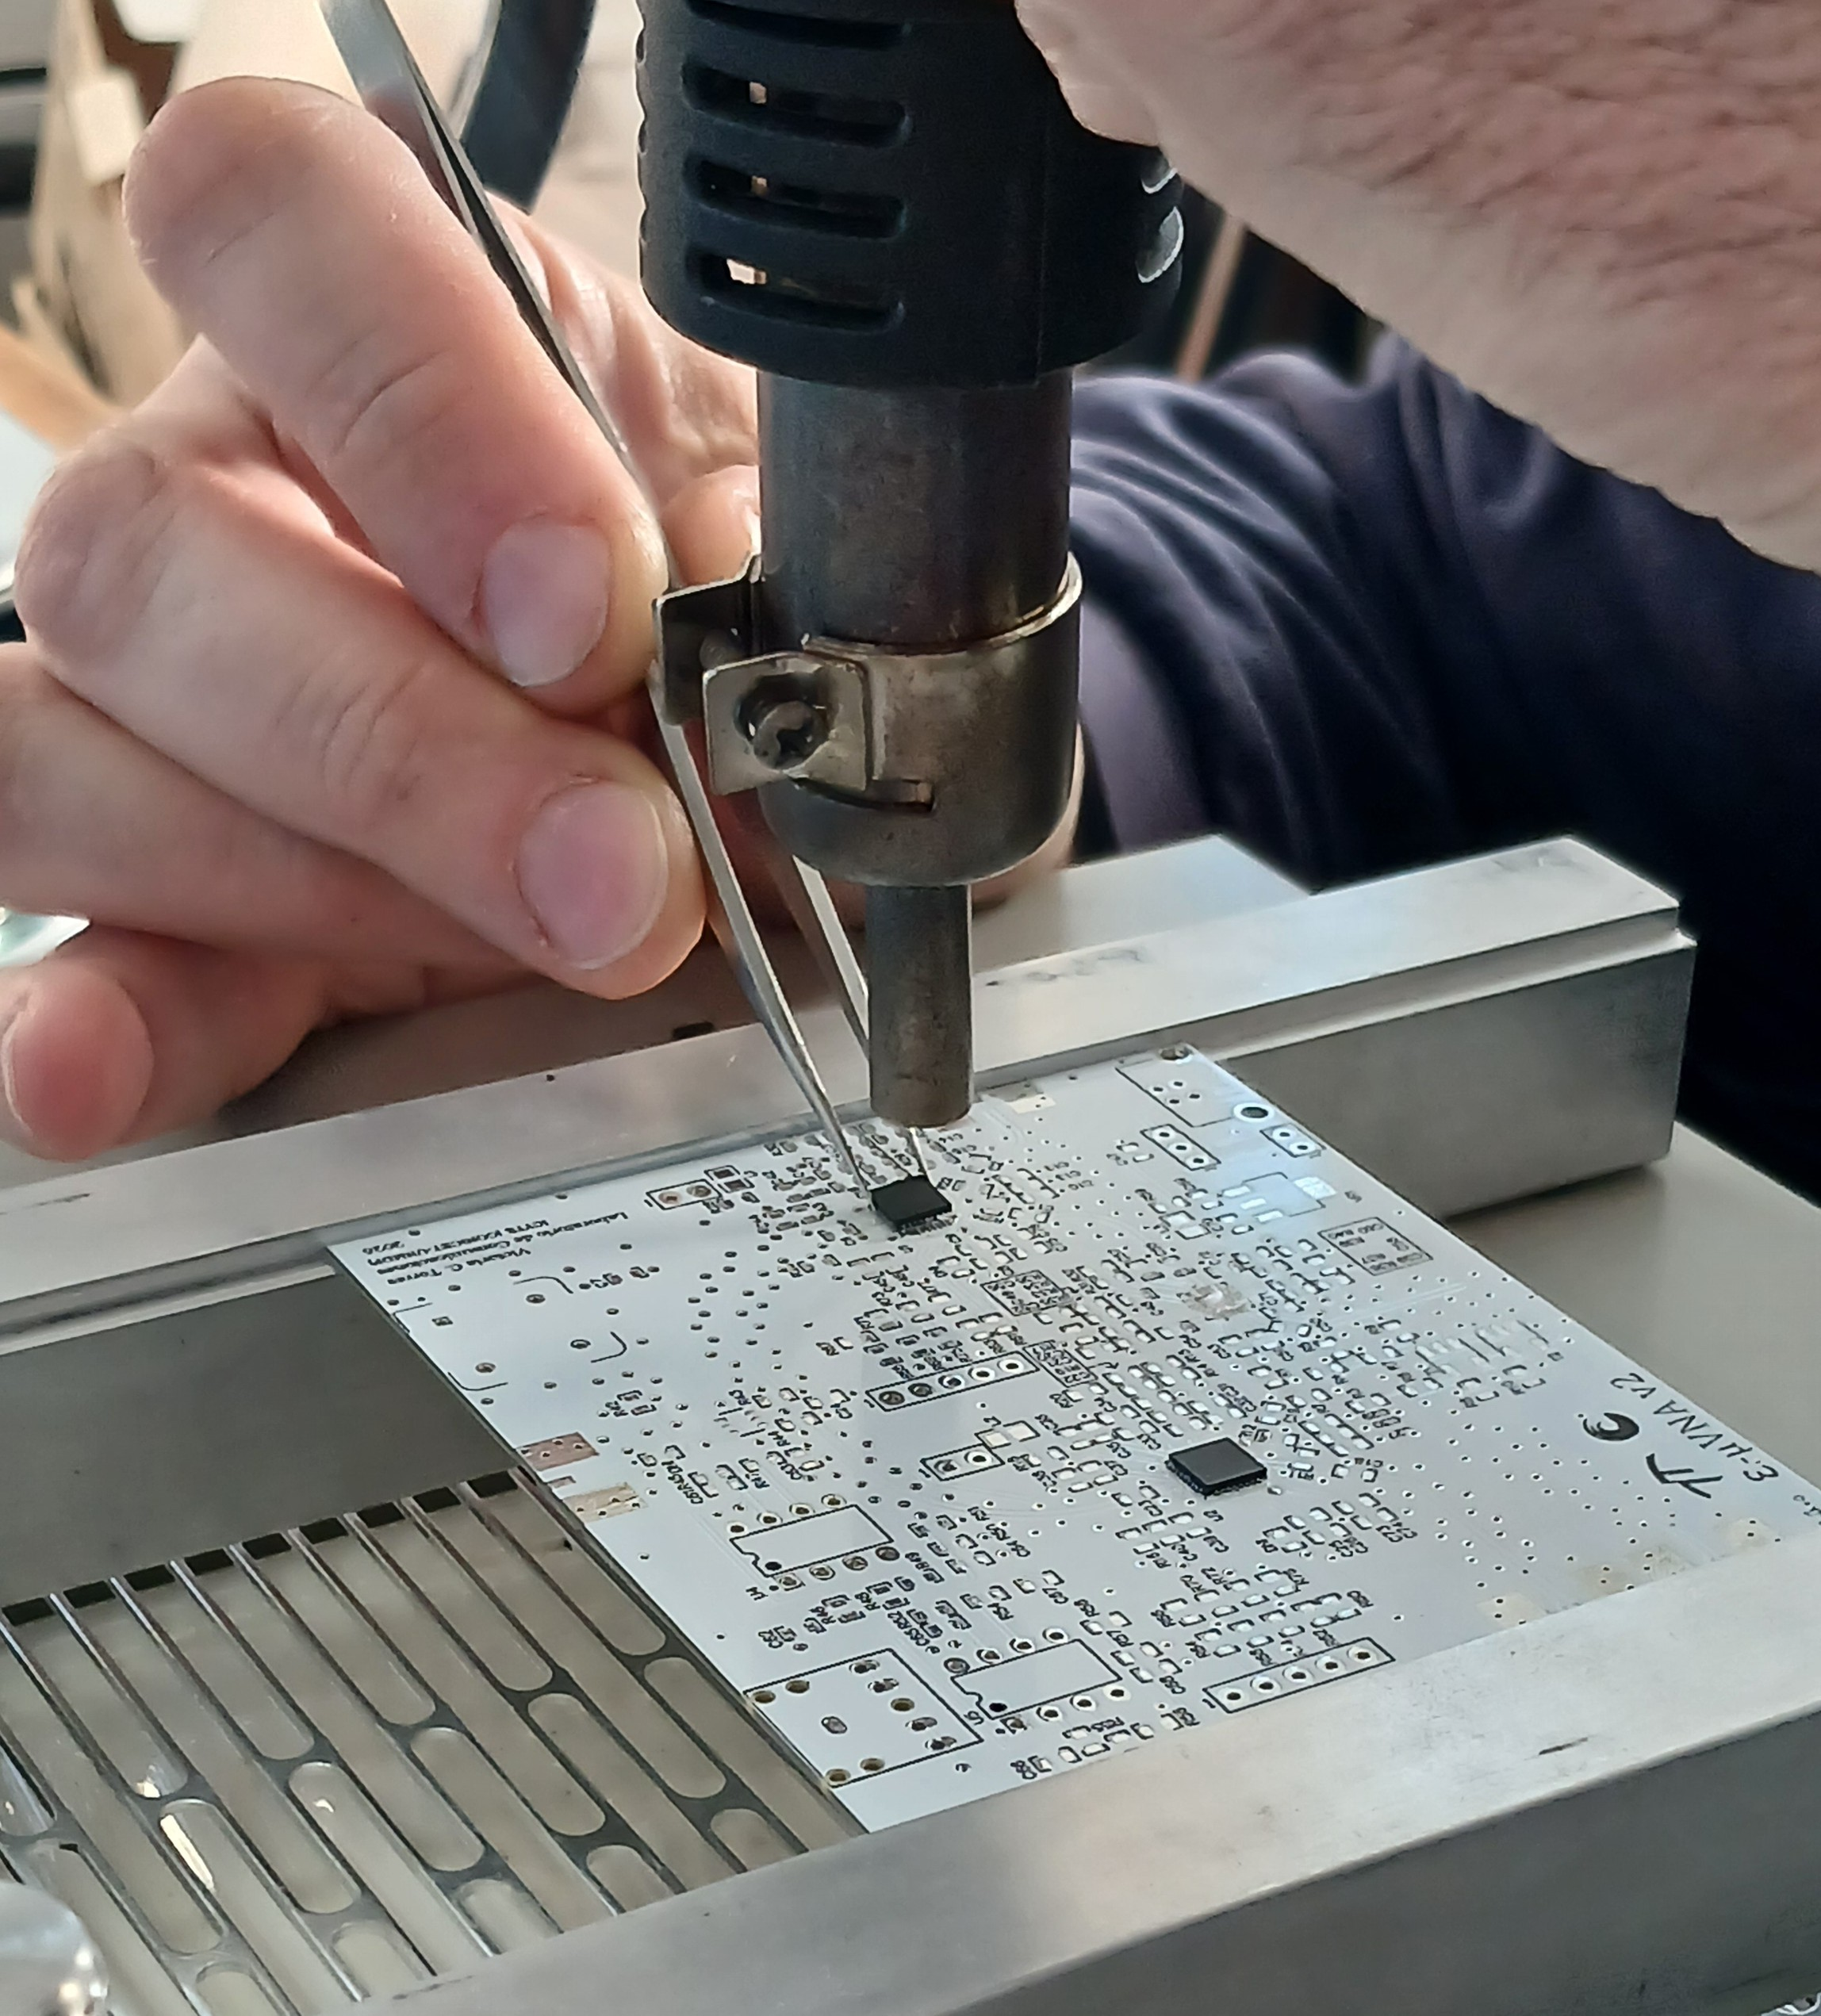
\includegraphics[width=0.5\linewidth]{Imagenes/soldadoqfn.jpg}
    \caption{Soldado de componentes QFN}
    \label{fig:qfn}
\end{figure}

Luego se soldaron el resto de componentes, en orden de menor a mayor altura. La figura \ref{fig:bancosoladado} exhibe el banco de soldado. La placa final se muestra en la figura \ref{fig:fotoplacafinal}. Es interesante destacar que debido al plano de masa continuo en la segunda capa, la placa posee muy buenos niveles de disipación, lo que dificultó considerablemente el proceso de soldado. Este inconveniente se resolvió mediante la combinación del uso de precalentadora, pistola de aire y soldador de lápiz simultáneamente y generosas cantidades de flux, como ilustra la figura \ref{fig:soldando}.

\begin{figure}
    \centering
    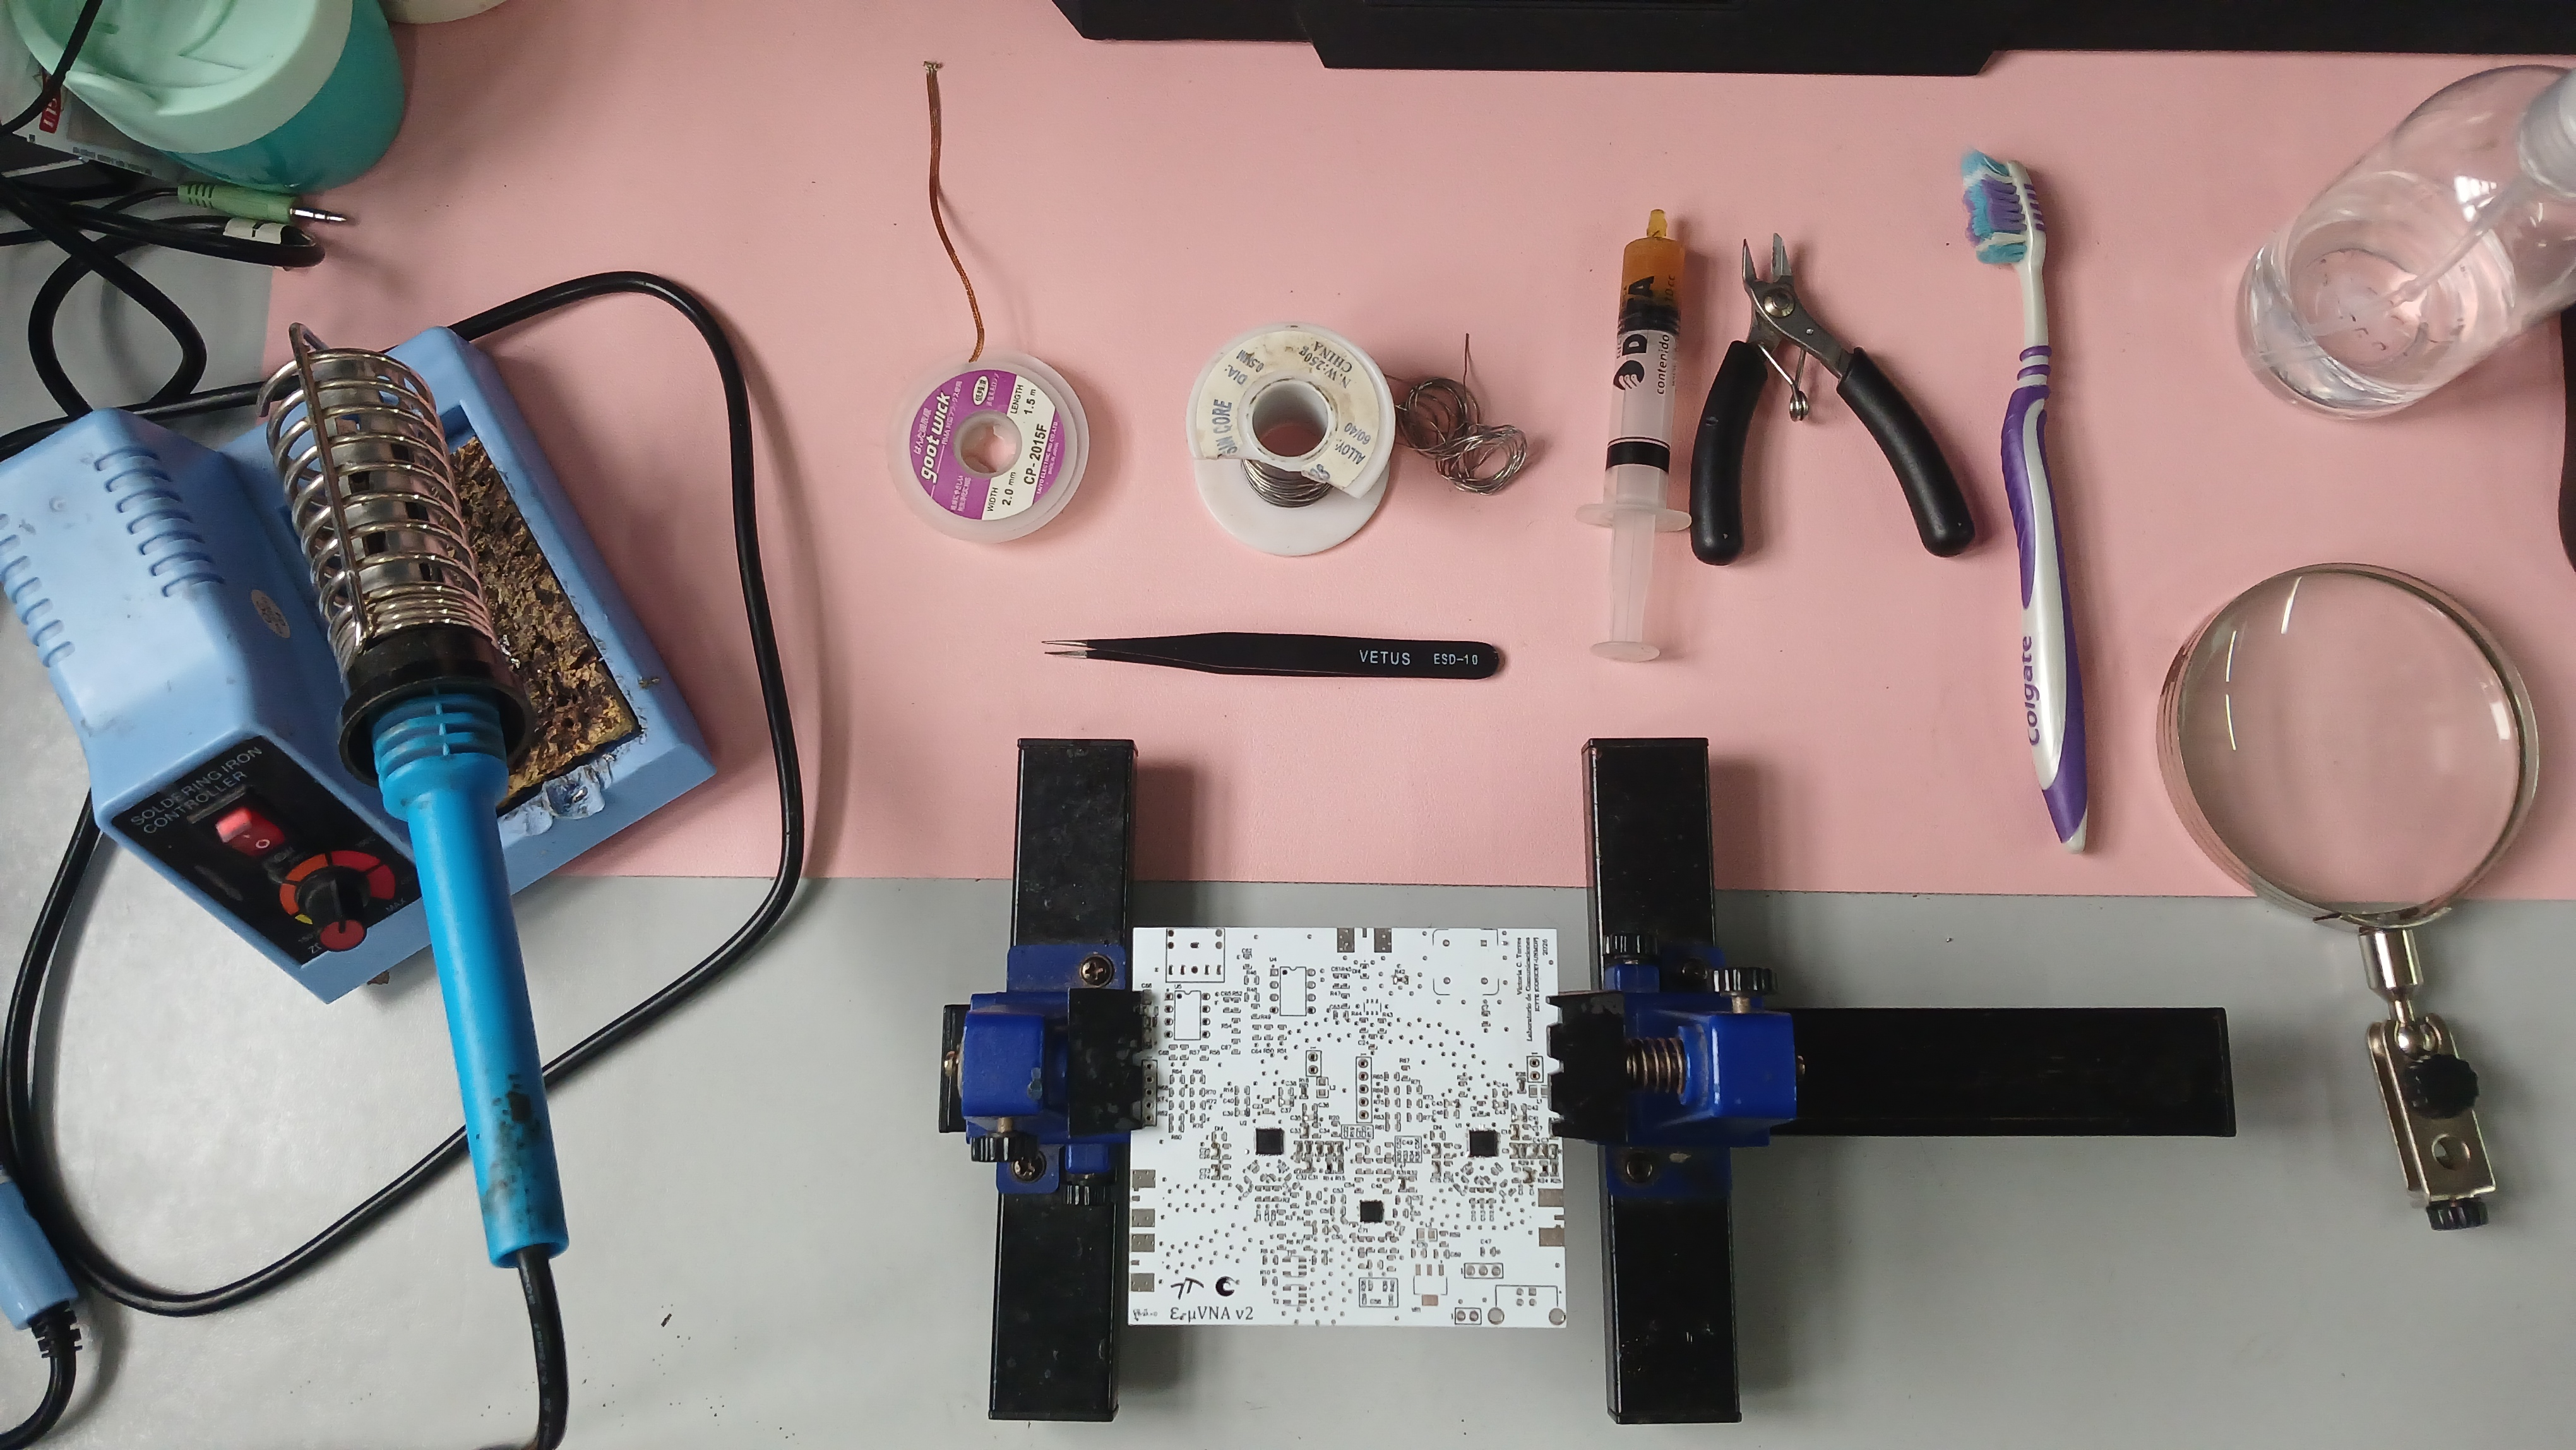
\includegraphics[width=0.9\linewidth]{Imagenes/bancosoldado2.jpg}
    \caption{Banco de soldado}
    \label{fig:bancosoladado}
\end{figure}

\begin{figure}[htbp]
    \centering
    \begin{minipage}[t]{0.48\textwidth}
        \centering
        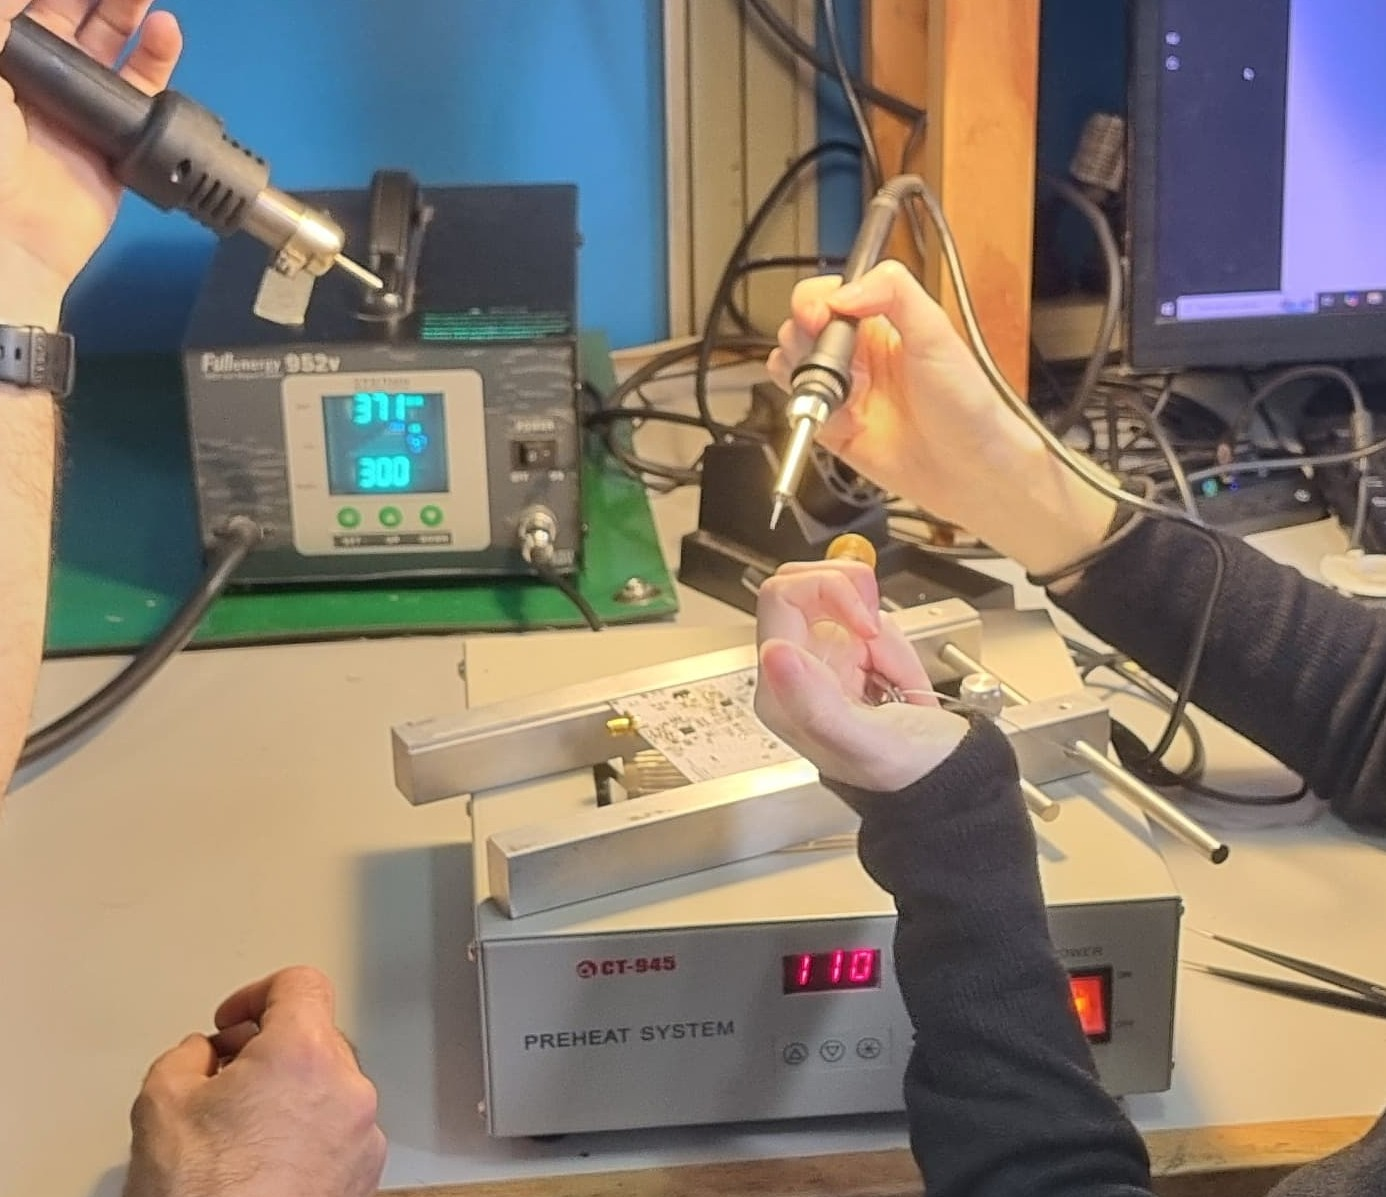
\includegraphics[width=\linewidth]{Imagenes/brianyyosoldando.jpg}
        \captionof{figure}{Proceso de soldado.}
        \label{fig:soldando}
    \end{minipage}
    \hfill
    \begin{minipage}[t]{0.48\textwidth}
        \centering
        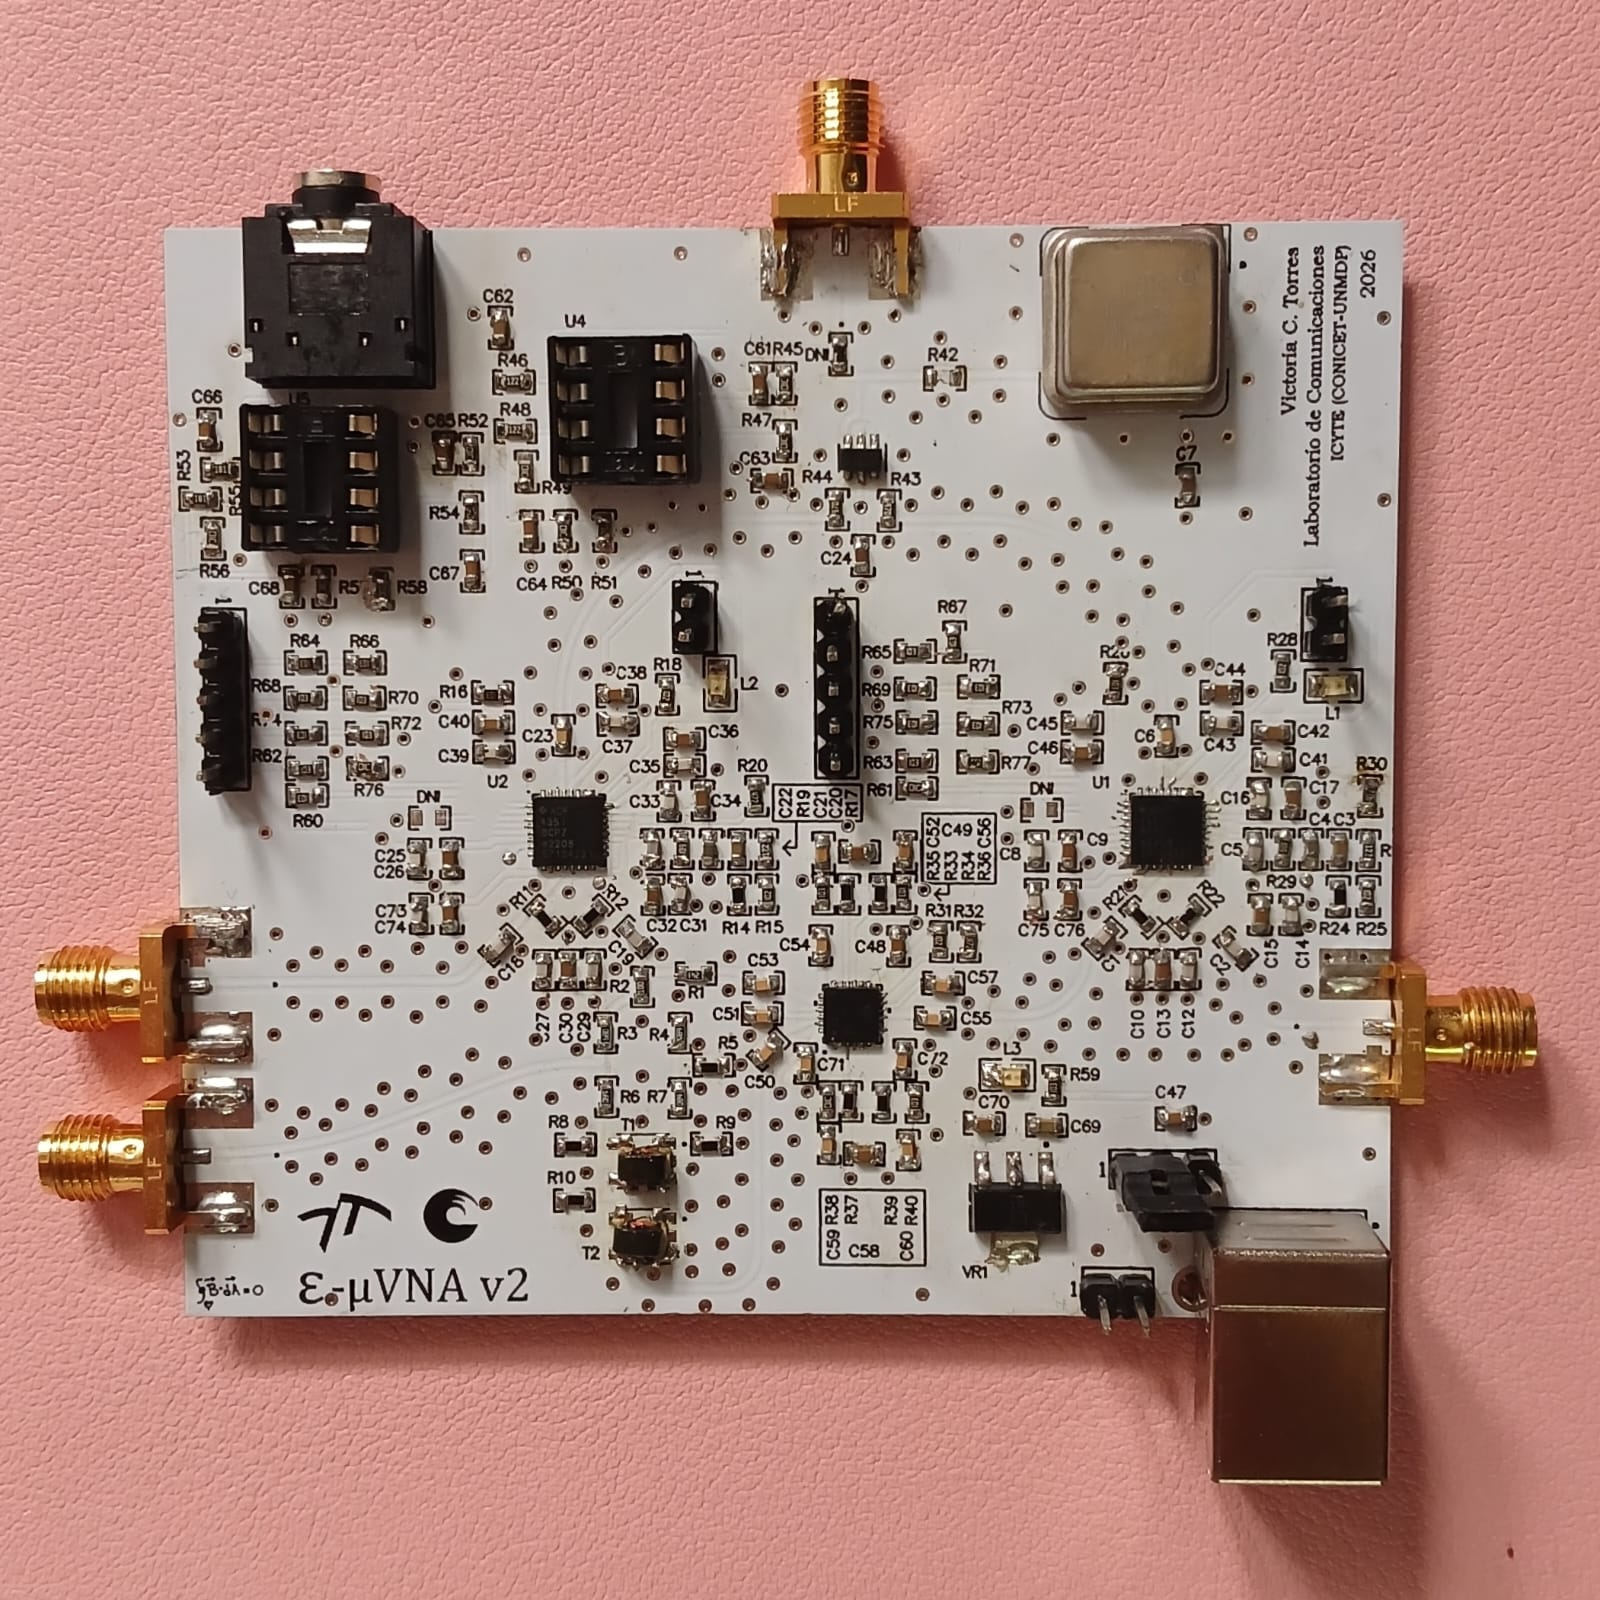
\includegraphics[width=\linewidth]{Imagenes/fotoplaca.jpeg}
        \captionof{figure}{$\epsilon\text{-}\mu\text{VNA}$ v2 final.}
        \label{fig:fotoplacafinal}
    \end{minipage}
\end{figure}

\section{Ficha técnica}
\begin{center}
\begin{tabularx}{\textwidth}{|X|X|X|}
\arrayrulecolor{Thistle}
\hline
\rowcolor{Thistle!20} 
\textbf{Parámetro}  & \textbf{Valor} & \textbf{Comentarios}  \\
\hline
Rango de frecuencia de trabajo & 1,8 a 2,2 GHz & Ampliable por software\\
\hline
Resolución (paso mínimo) en RF & 250 Hz & En la banda de trabajo. Según la hoja de datos del AF4351, el mínimo con este hardware sería 31,25 Hz pero no se han hecho pruebas.\\
\hline
Impedancia característica & $50 \Omega$ & -\\
\hline
Directividad del acoplador resistivo & >36,5 dB & Para el rango de frecuencia de trabajo \\
\hline
Voltaje de alimentación & 5V & Vía USB-B o fuente externa\\
\hline
Corriente de alimentación & 350 mA & - \\
\hline
Frecuencia de muestreo & 44,1 kHz & Configurable por software \\
\hline
Resolución del ADC (placa de sonido) & 16 bits & Entrada Line-In de la PC \\
\hline
Baud rate (microcontrolador) & 115200 baudios & Configurable \\ 
\hline

\end{tabularx}
\end{center}

\section{Pruebas de integración}
Para verificar el correcto funcionamiento de la placa, la primera prueba unitaria realizada fue medir la entrada y salida del regulador de tensión. Se verificó que hubieran 5 V y 3,3 V respectivamente.

Se midió la frecuencia del cristal con un frecuencímetro Optoelectronics Handi-Counter 2810 \cite{optoelectronics_2810_manual}, alimentando el oscilador con fuente de alimentación regulable Kenwood PA36-3A \cite{kenwood_pa36_3a}. Como evidencia la figura \ref{fig:med_cristal}, el cristal es de 10 MHz.
\begin{figure}
    \centering
    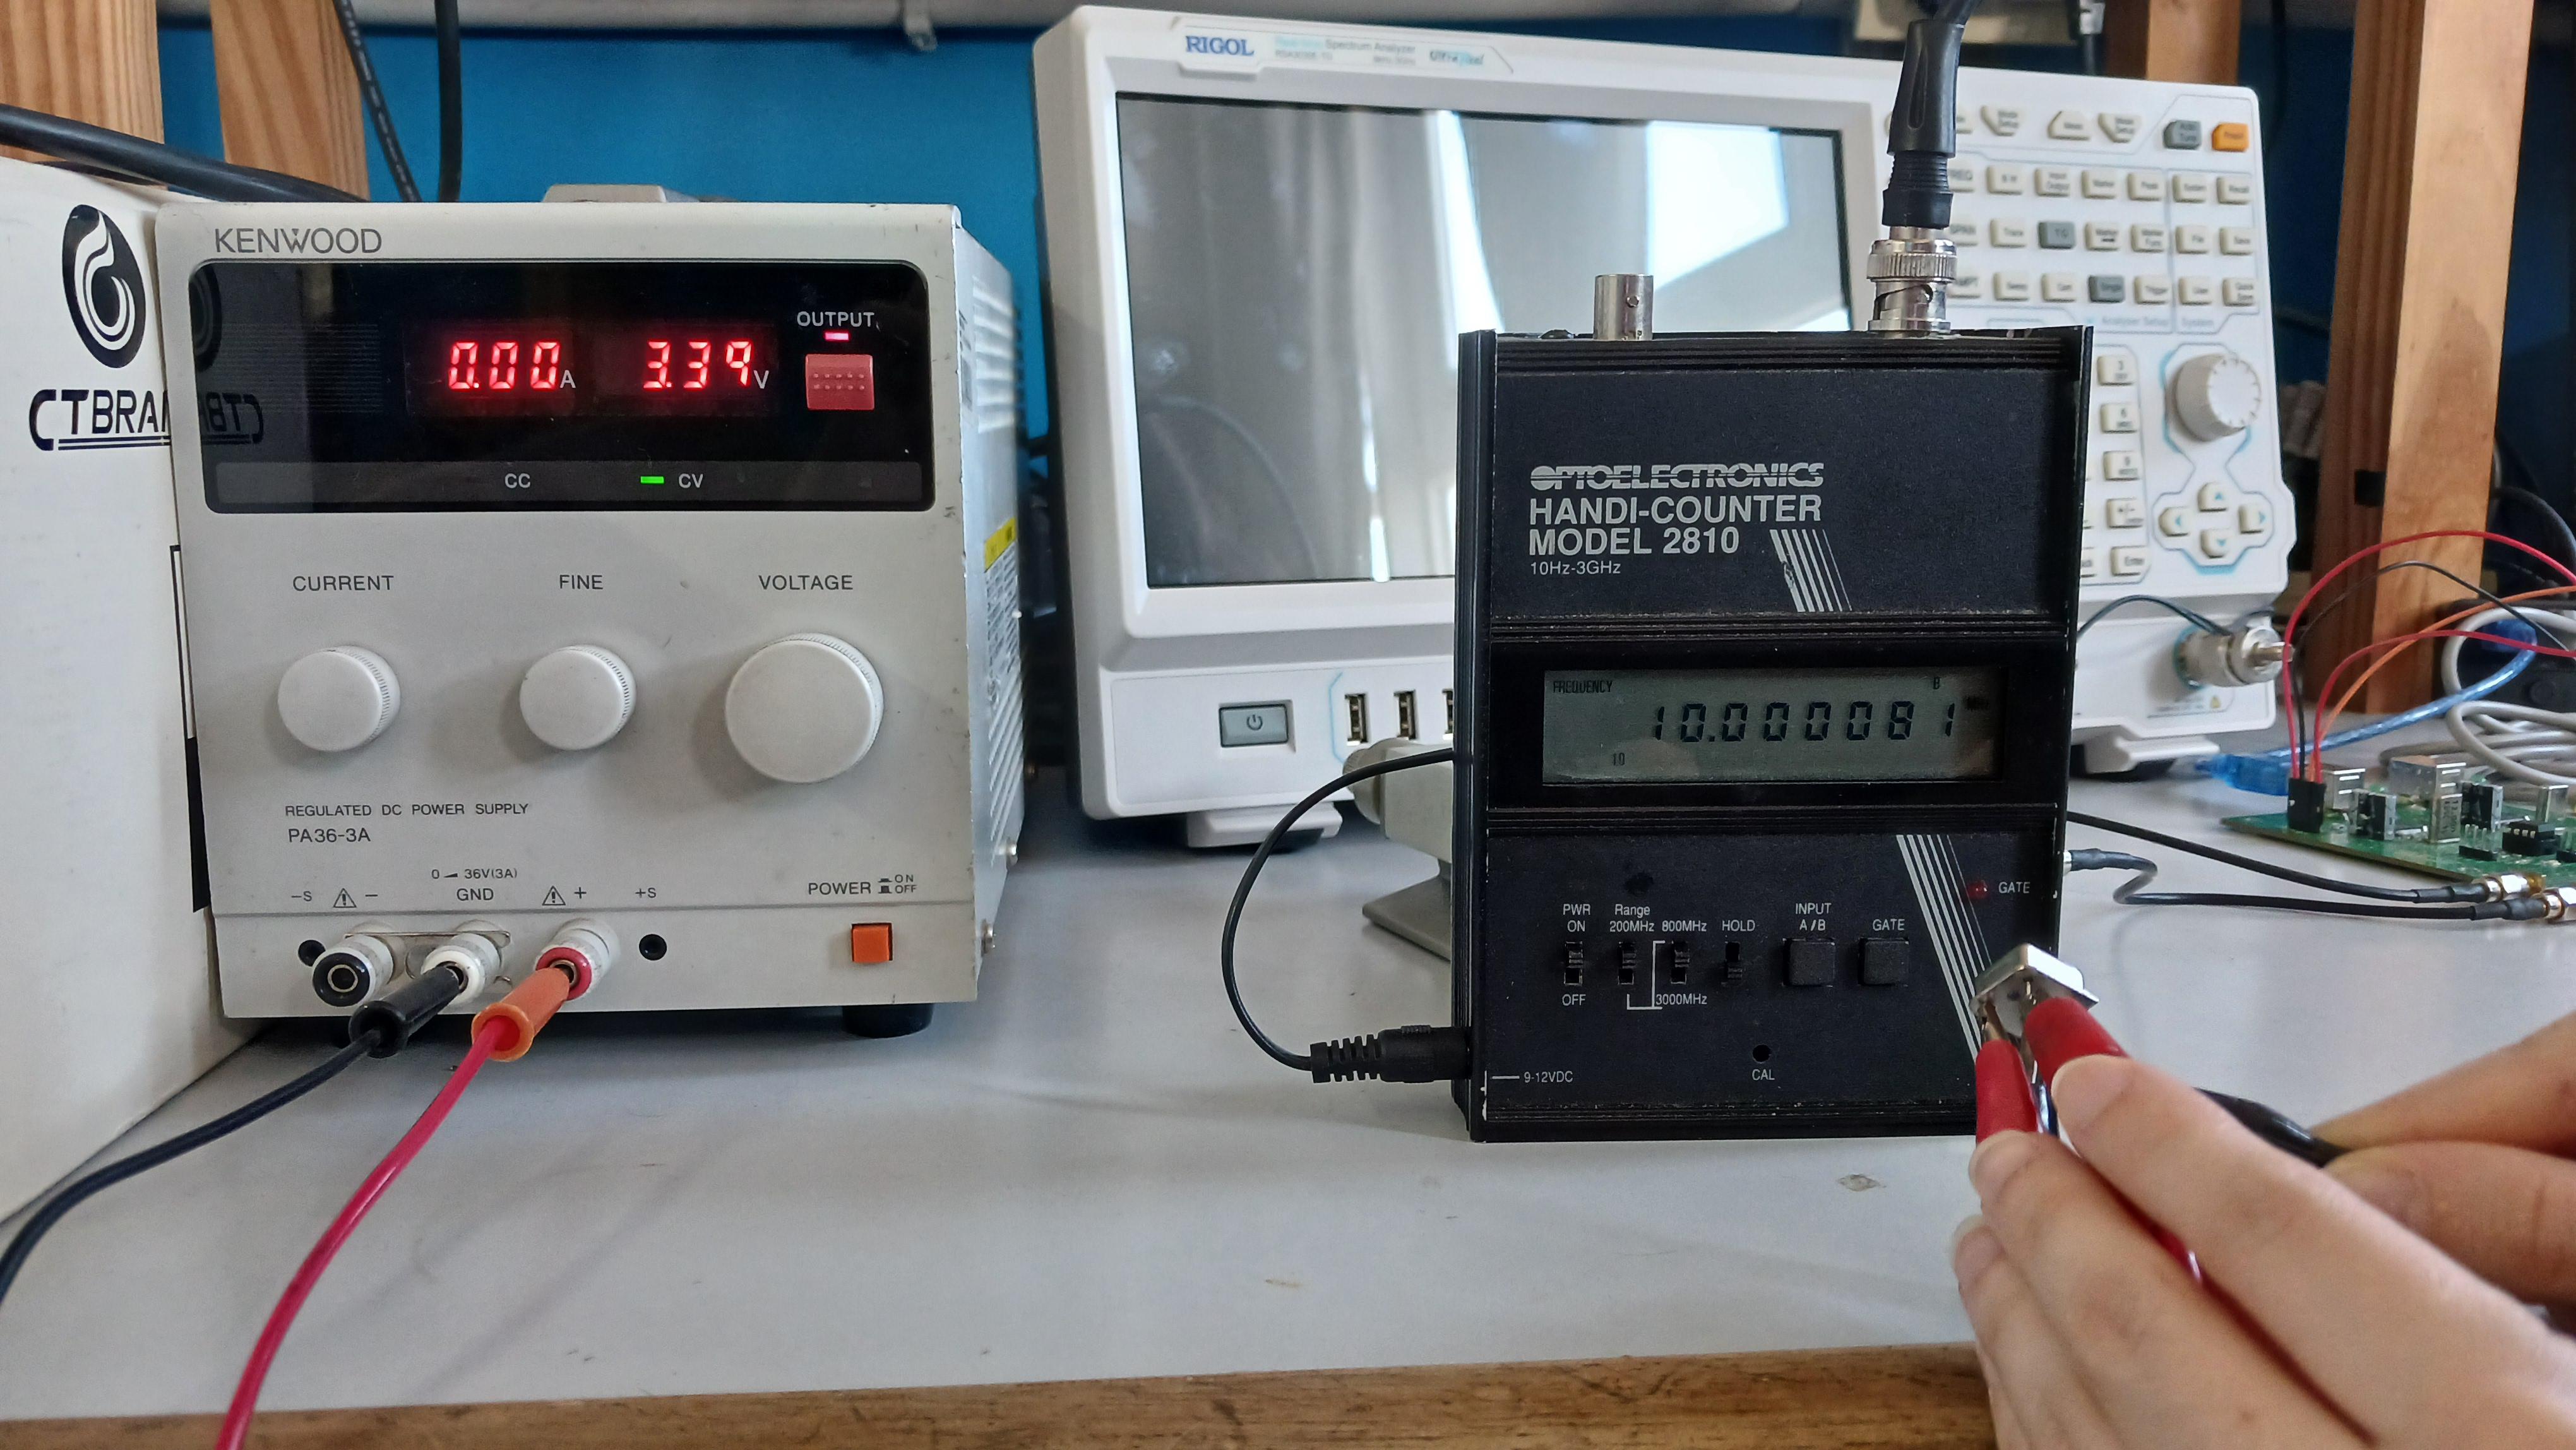
\includegraphics[width=0.6\linewidth]{Imagenes/pruebacristal.jpg}
    \caption{Banco de medición de la frecuencia del oscilador a cristal.}
    \label{fig:med_cristal}
\end{figure}

Luego se programó la generación de una única señal para cada generador de RF y así comprobar el enganche y el nivel de potencia de salida. Para esta medición se utilizaron las salidas auxiliares con conectores SMA. El banco de medición (véase la figura \ref{fig:bancomed_1frec}) consistió en la fuente regulable para alimentar la placa, una PC para programar el Arduino, un analizador de espectros Rigol RSA3030N \cite{rigol_rsa3030n}, y un atenuador HP 8496B \cite{hp8496b_manual}, que se utilizó para proteger la entrada del analizador.

\begin{figure}
    \centering
    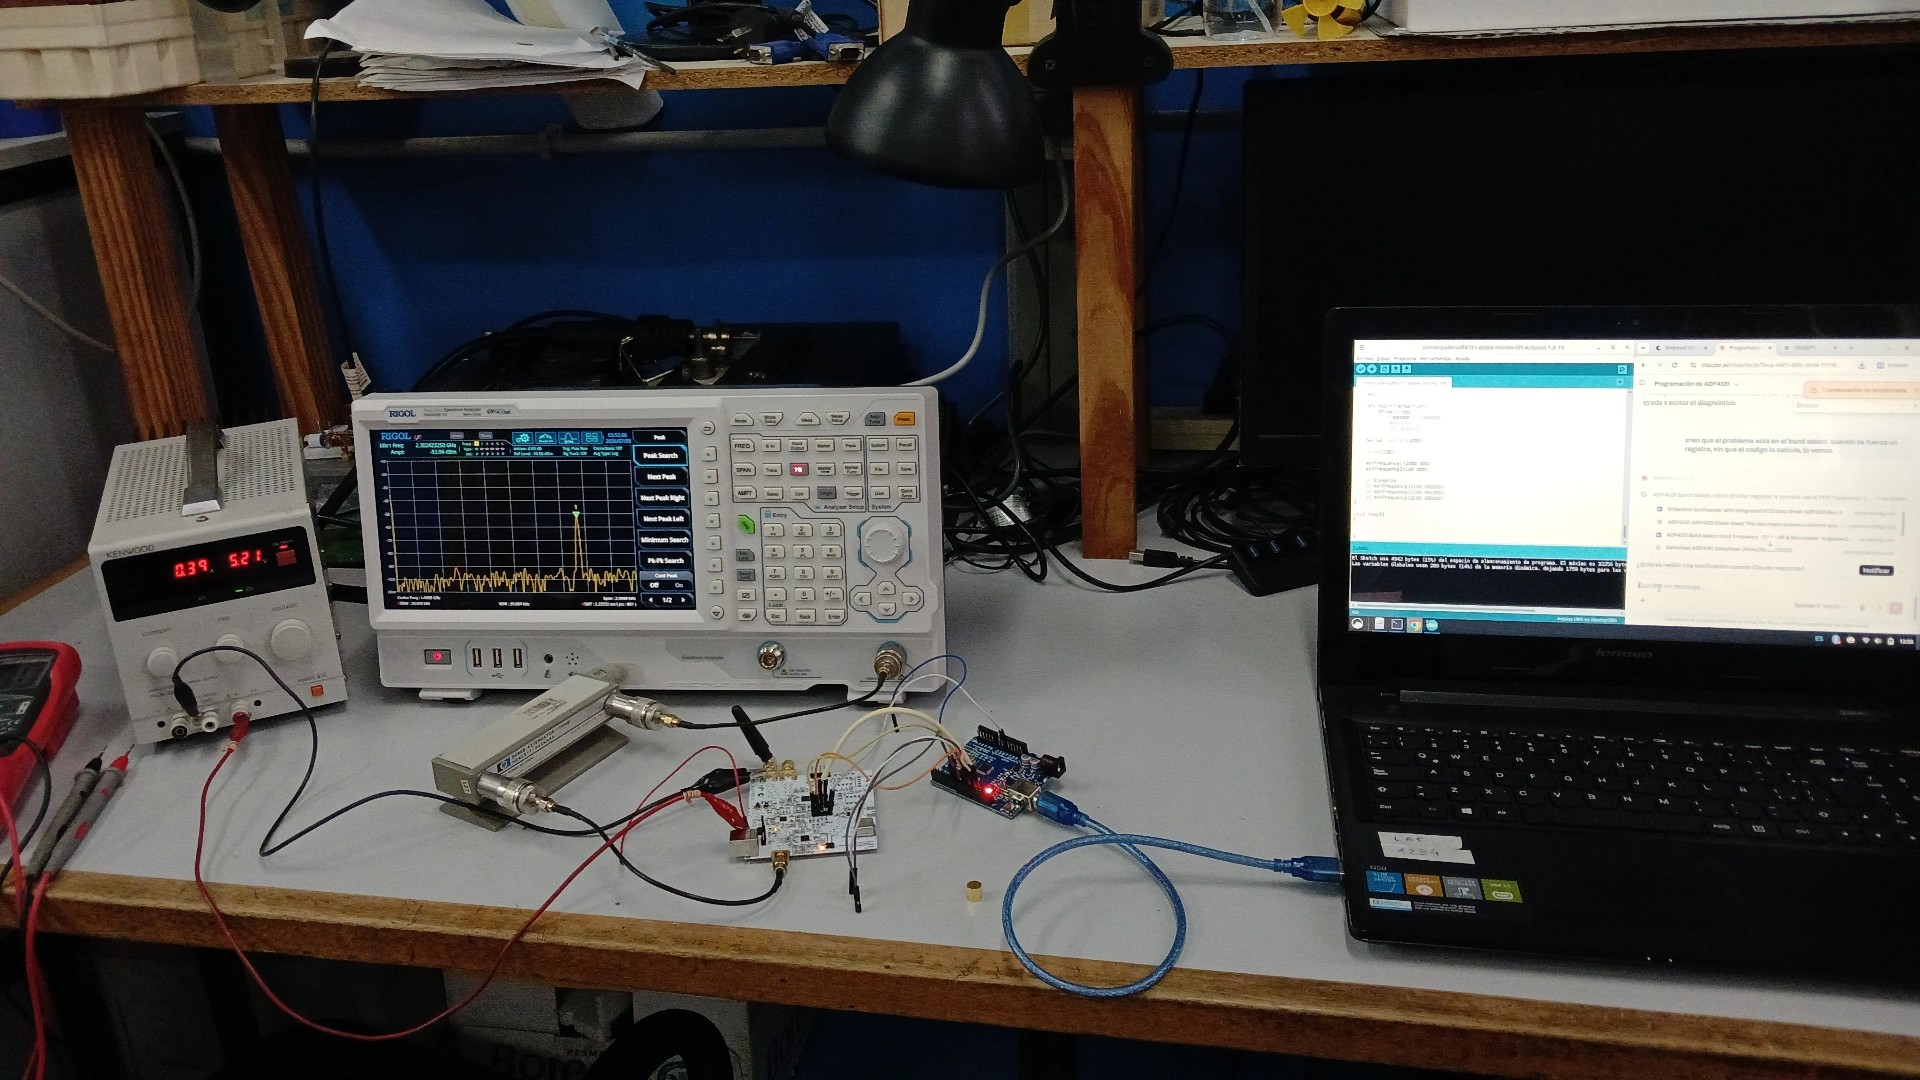
\includegraphics[width=0.7\linewidth]{Imagenes/banco_gen1frec.jpg}
    \caption{Banco de medición para generación de una única frecuencia.}
    \label{fig:bancomed_1frec}
\end{figure}

Con el mismo banco de medición, pero ajustando el programa del Arduino se generaron varios barridos de diferente frecuencia inicial, final y paso para verificar el enganche en toda la banda de interés, para ambos ADF4351.

Luego de comprobar con éxito el funcionamiento de estos subsistemas, se soldó la etapa de FI para avanzar hacia la adquisición. Para probar la placa de sonido, se generaron dos frecuencias separadas en 1, 5 y 10 kHz. Se adquirieron con el software Audacity \cite{audacity376} en modo estéreo, como muestran las figuras \ref{fig:audacity}. Se eligió como FI de trabajo 10 kHz (figura \subref{fig:grab10k}) porque una mayor FI reduce el ruido de fase y está alejada de las zonas de ruido de baja frecuencia (ruido de red y 1/f), pero los pasa bajos a la salida del mezclador limitan la frecuencia máxima que se puede elegir. 

\begin{figure}[htbp]
    \centering
    \begin{subfigure}[b]{0.8\textwidth}
        \centering
        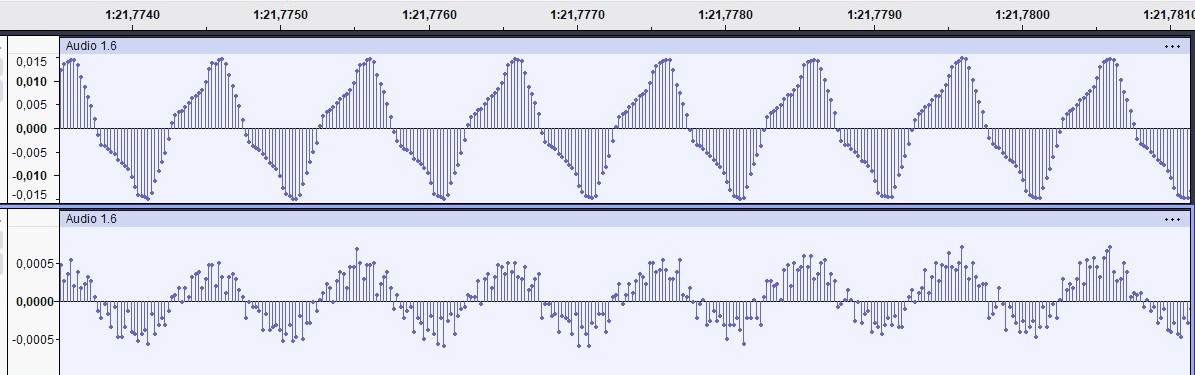
\includegraphics[width=\textwidth]{Imagenes/grabación 1 k.jpg}
        \caption{Grabación con FI = 1 kHz.}
        \label{fig:grab1k}
    \end{subfigure}

    \vspace{1em}   % espacio entre subfiguras (opcional)

    \begin{subfigure}[b]{0.8\textwidth}
        \centering
        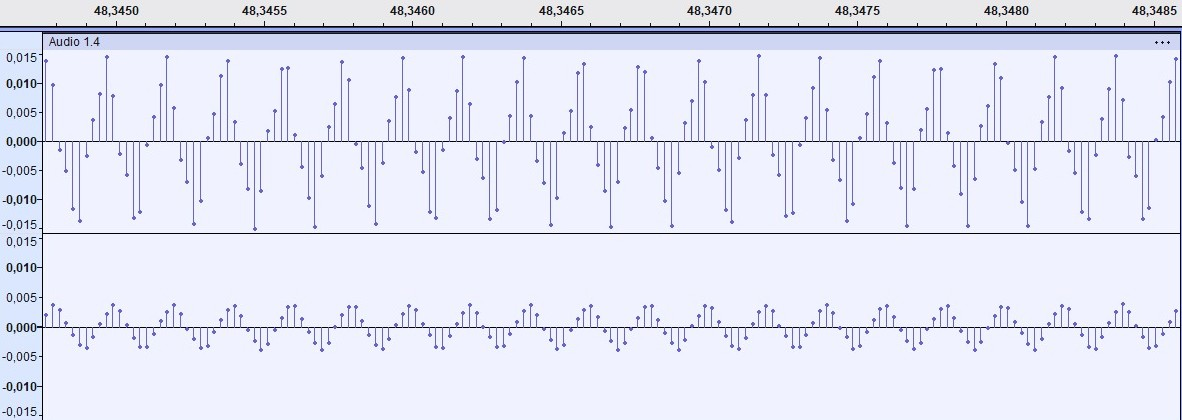
\includegraphics[width=\textwidth]{Imagenes/Grabación 5k.jpg}
        \caption{Grabación con FI = 5 kHz.}
        \label{fig:grab5k}
    \end{subfigure}

    
    \begin{subfigure}[b]{0.8\textwidth}
        \centering
        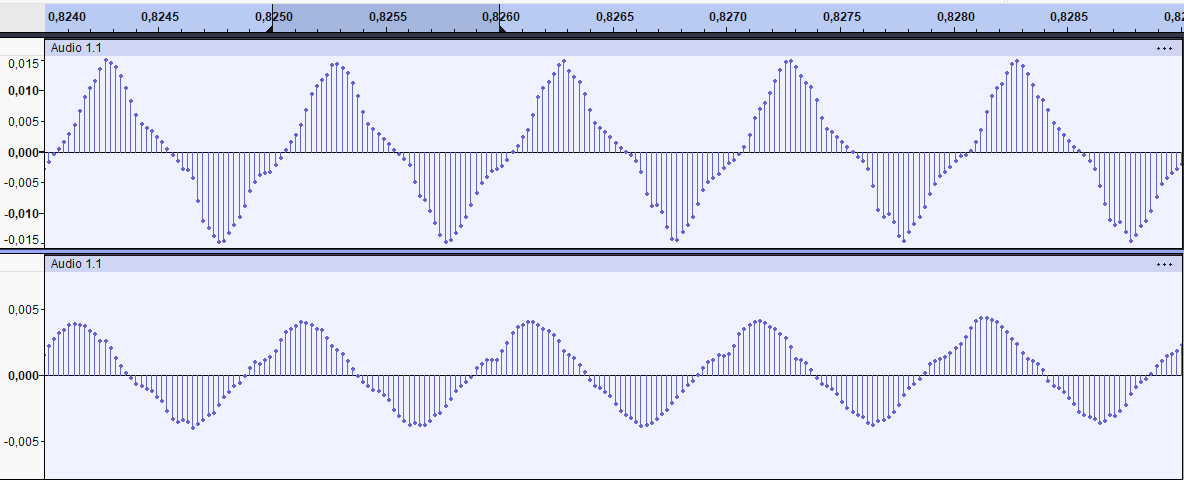
\includegraphics[width=\textwidth]{Imagenes/grabación 10k.png}
        \caption{Grabación con FI = 10 kHz.}
        \label{fig:grab10k}
    \end{subfigure}

    \caption{Grabaciones de prueba en Audacity.}
    \label{fig:audacity}
\end{figure}

El mismo software tiene una herramienta para graficar el espectro de la señal, en el que se pudo comprobar la frecuencia de mayor amplitud y comprobar que el tercer armónico queda aproximadamente 13 dB por debajo del primero, como indica la hoja de datos de los ADF4351 y como se muestra en la figura \ref{fig:espectro1k}.

\begin{figure}
    \centering
    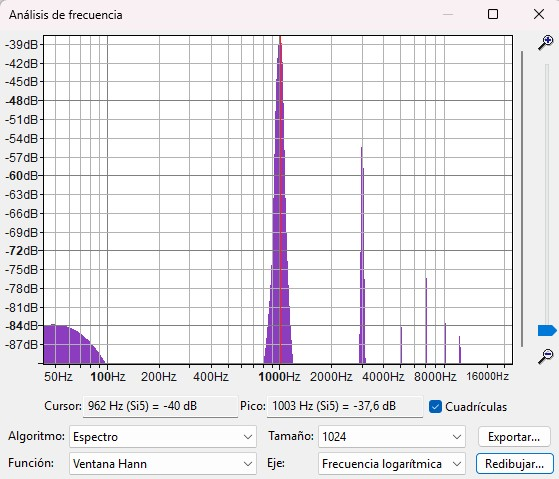
\includegraphics[width=0.6\linewidth]{Imagenes/espectro1kaudacity.jpg}
    \caption{Espectro de la señal de referencia en una grabación con FI = 1 kHz.}
    \label{fig:espectro1k}
\end{figure}

Se procedió a probar una parte del software que aplicara el algoritmo de barrido y extracción del S11 sin calibrar. Las figuras \ref{fig:precalibracion} muestran la medición de una carga de 5O $\Omega$ y un cortocircuito. 

\begin{figure}[htbp]
    \centering
    \begin{subfigure}[b]{0.8\textwidth}
        \centering
        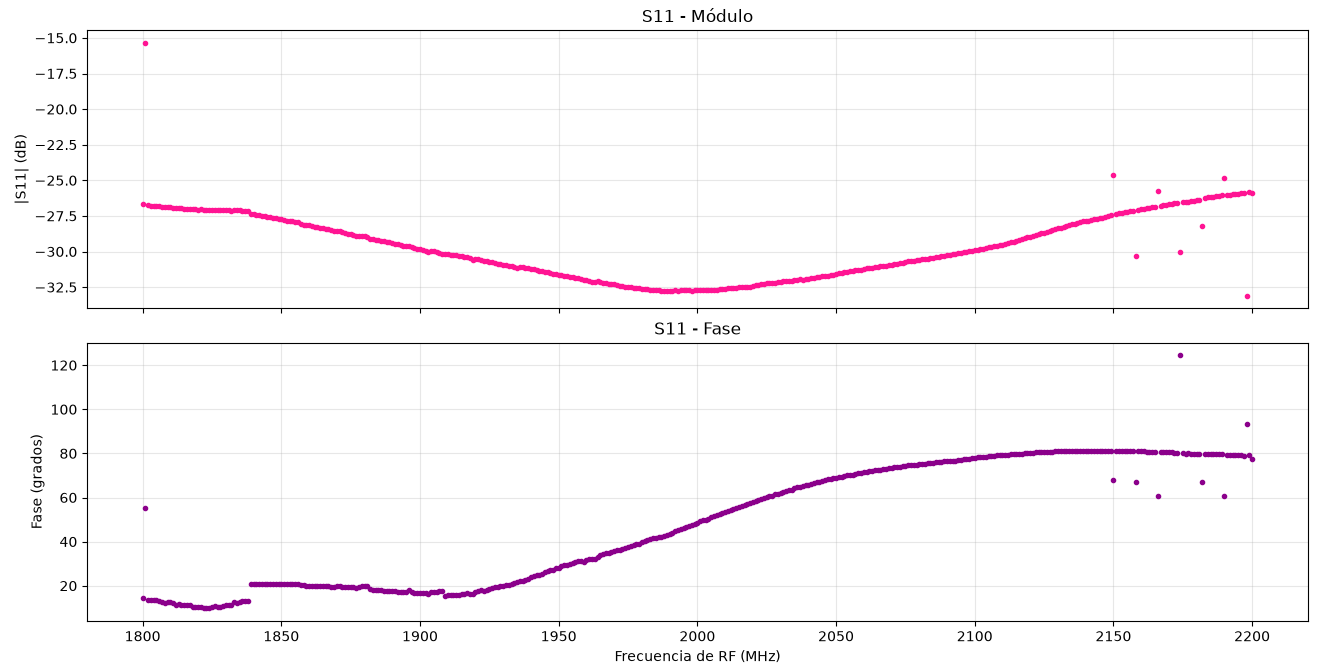
\includegraphics[width=\textwidth]{Imagenes/carga 50 sin calibrar.png}
        \caption{Medición de carga adaptada pre calibración.}
        \label{fig:50precalib}
    \end{subfigure}

    \vspace{1em}   % espacio entre subfiguras (opcional)
    
    \begin{subfigure}[b]{0.8\textwidth}
        \centering
        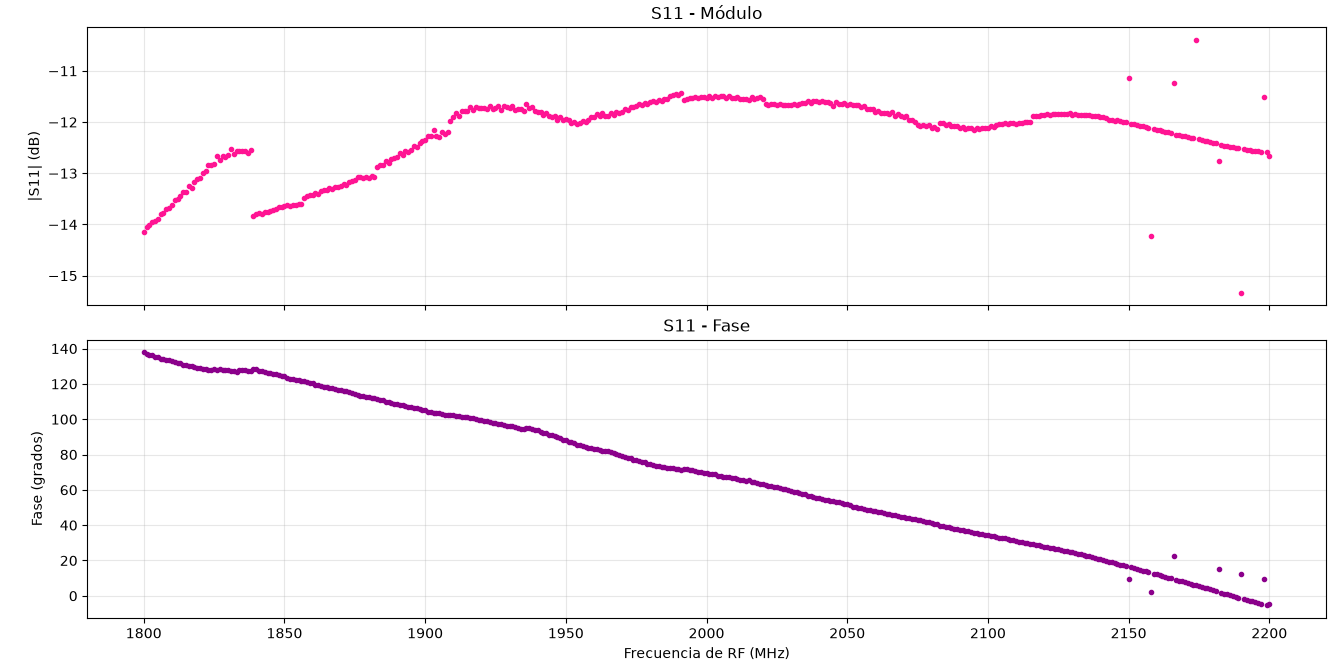
\includegraphics[width=\textwidth]{Imagenes/cortoprecalib.png}
        \caption{Medición de cortocircuito pre calibración.}
        \label{fig:cortoprecalib}
    \end{subfigure}
    \label{fig:precalibracion}

\end{figure}


Se puede observar que aunque las mediciones tienen coherencia en cuanto a la forma (exceptuando algunas regiones), los valores de amplitud y fase medidos no son los correctos. Esto se debe a los errores que se mencionaron en la sección \ref{sec:errores}, que se reducen mediante la calibración. 


\section{Mediciones de sistemas bajo prueba}

Por último, se probó el software completo, incluyendo la calibración SOL, para varios DUT:

\subsection{Cortocircuito}
Es el unico que medi la carga de calibracion porque no tenia otro corto que no sea el de 150.
\subsubsection{Cortocircuito de 150°}
\begin{figure}
    \centering
    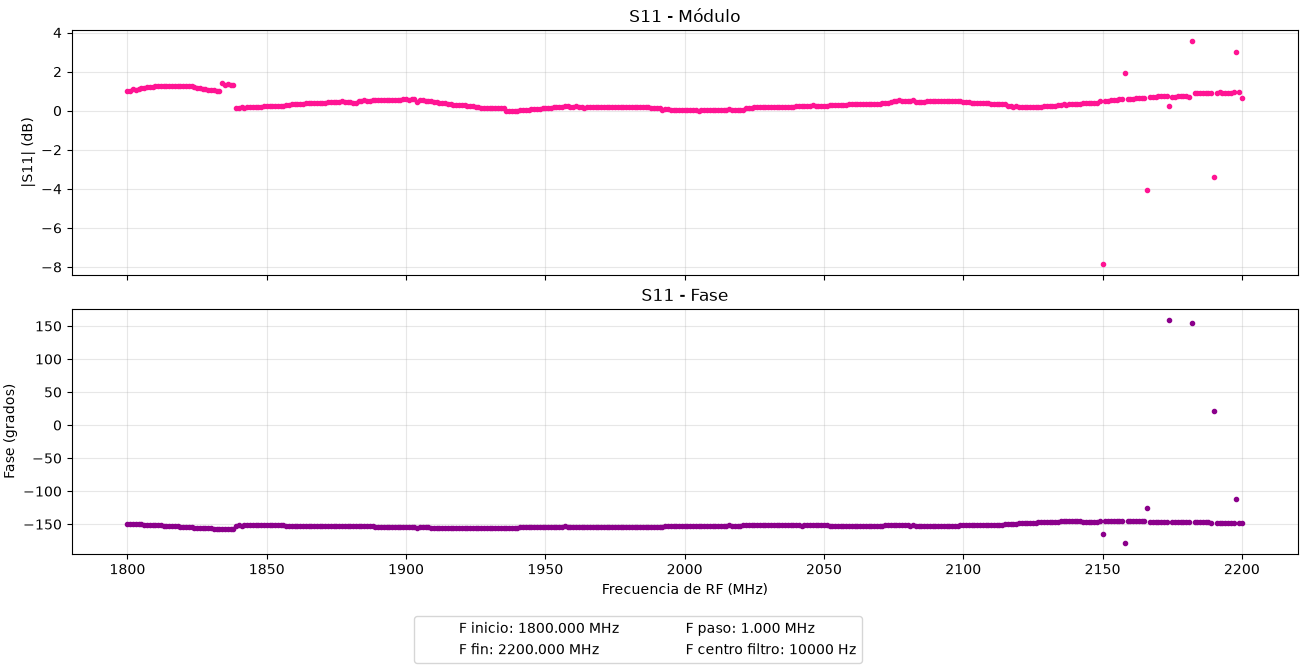
\includegraphics[width=0.7\linewidth]{Imagenes/medcorto150.png}
    \caption{Medición de cortocircuito.}
    \label{fig:med50R}
\end{figure}

\subsection{Circuito abierto}

\begin{figure}
    \centering
    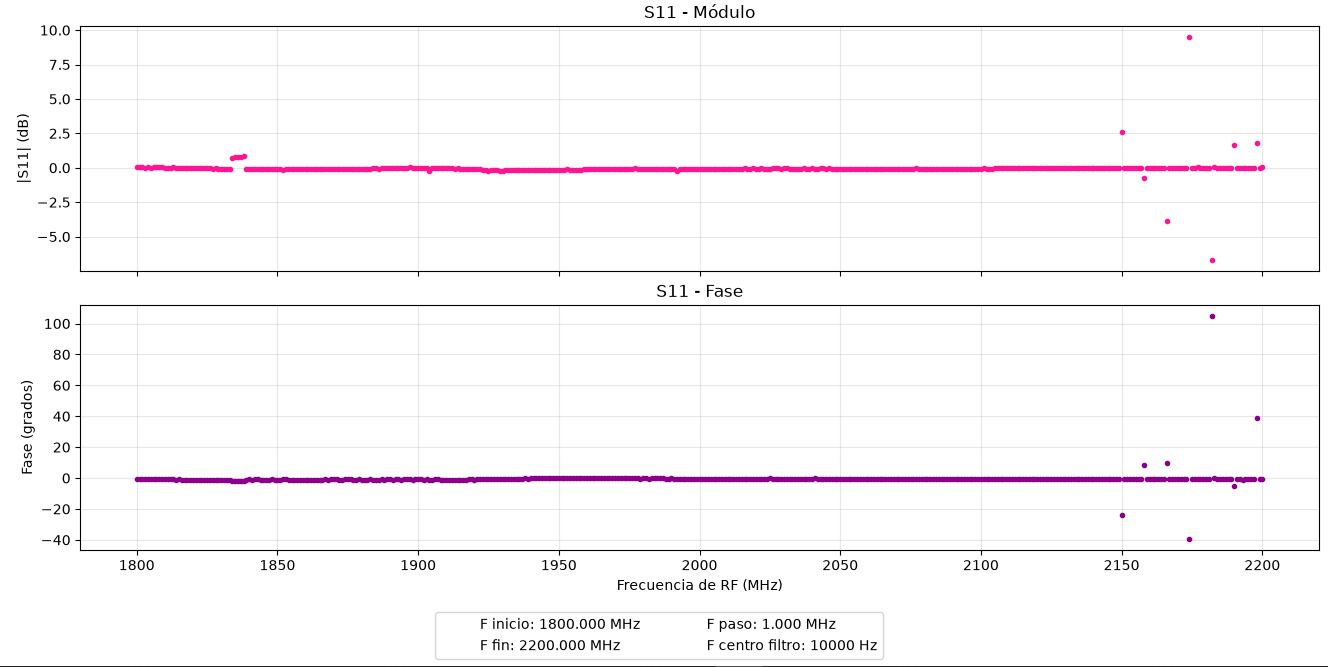
\includegraphics[width=0.7\linewidth]{Imagenes/medCA.png}
    \caption{Medición de 50 $\Omega$.}
    \label{fig:med50R}
\end{figure}

\subsection{Adaptación (50 $\Omega$)}

\begin{figure}
    \centering
    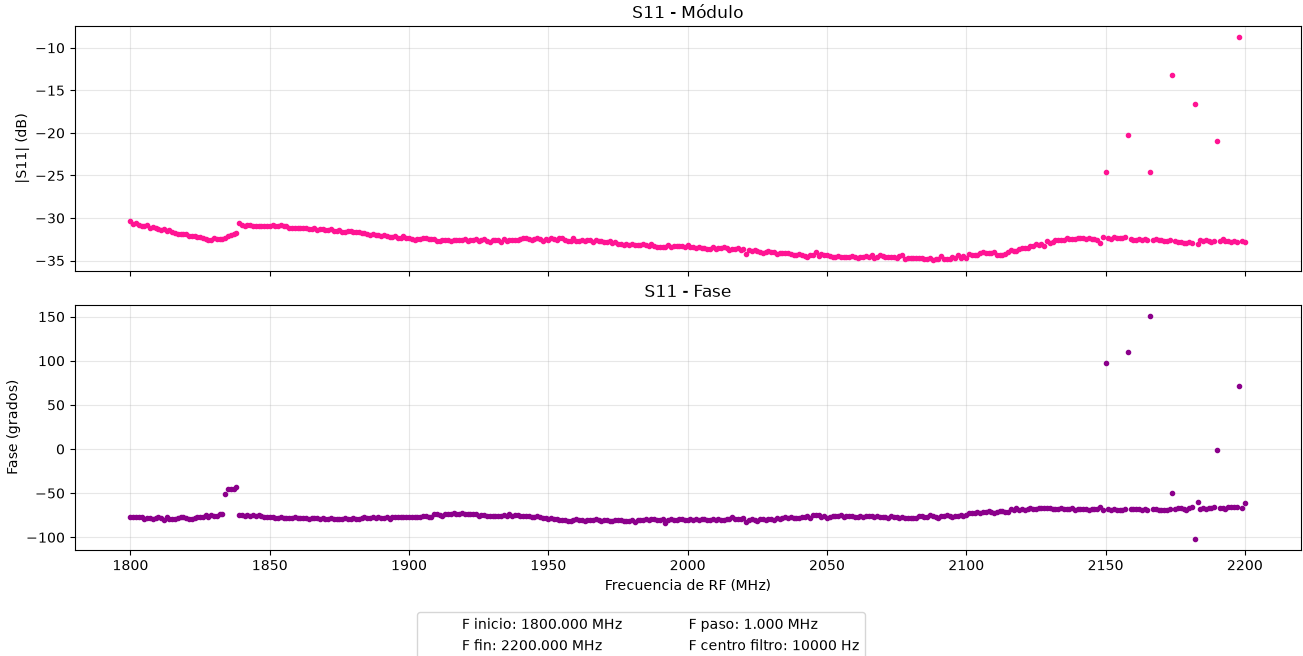
\includegraphics[width=0.7\linewidth]{Imagenes/med50R.png}
    \caption{Medición de 50 $\Omega$.}
    \label{fig:med50R}
\end{figure}

La siguiente tabla muestra una comparación entre los coeficientes de reflexión teóricos o "reales" y el promedio (aproximado) de los medidos, en módulo [dB] y ángulo [°]:
\begin{center}
\begin{tabularx}{\textwidth}{|X|X|X|}
\arrayrulecolor{Thistle}
\hline
\rowcolor{Thistle!20} 
\textbf{Carga}  & \textbf{$\Gamma_{REAL}$} & \textbf{$\Gamma_{MEDIDO}$}  \\
\hline
50 $\Omega$ & - $\inf$ & -32,5 \\
\hline
68 $\Omega$ & -16,33 $\angle$ 0 & -15,8 $\angle$ 6 \\
\hline
Corto circuto & 0 $\angle$ 180 & \\
\hline
Circuito abierto & 0 $\angle$ 0 & 0 $\angle$ 0 \\
\hline
Cortocircuito de 150° & 0 $\angle$ 150 & \\
\end{tabularx}
\end{center}

\subsection{Sensor resonante}
Finalmente, para verificar que el sistema está adaptado para operar en conjunto con un sensor de glucemia no invasivo, se utiliza el sensor que resuena alrededor de los 2 GHz. Se mide en principio en vacío, como muestra la figura \ref{fig:sensorvacio}.  

\begin{figure}
    \centering
    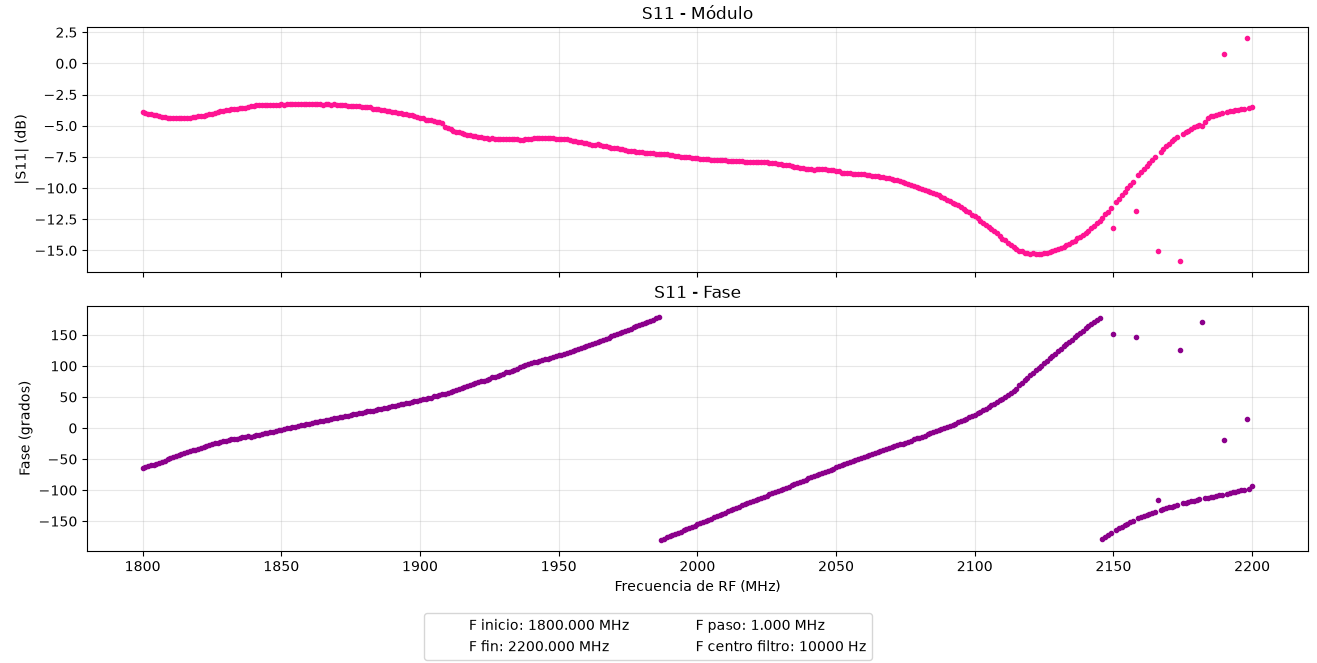
\includegraphics[width=0.7\linewidth]{Imagenes/sensor_vacio.png}
    \caption{Medición del sensor de glucemia en vacío.}
    \label{fig:sensorvacio}
\end{figure}

Si se introduce en el sensor un dedo, debería moverse la frecuencia de resonancia por lo explicado en el capítulo 1. Se confirma este comportamiento en la figura \ref{fig:sensorlleno}

\begin{figure}
    \centering
    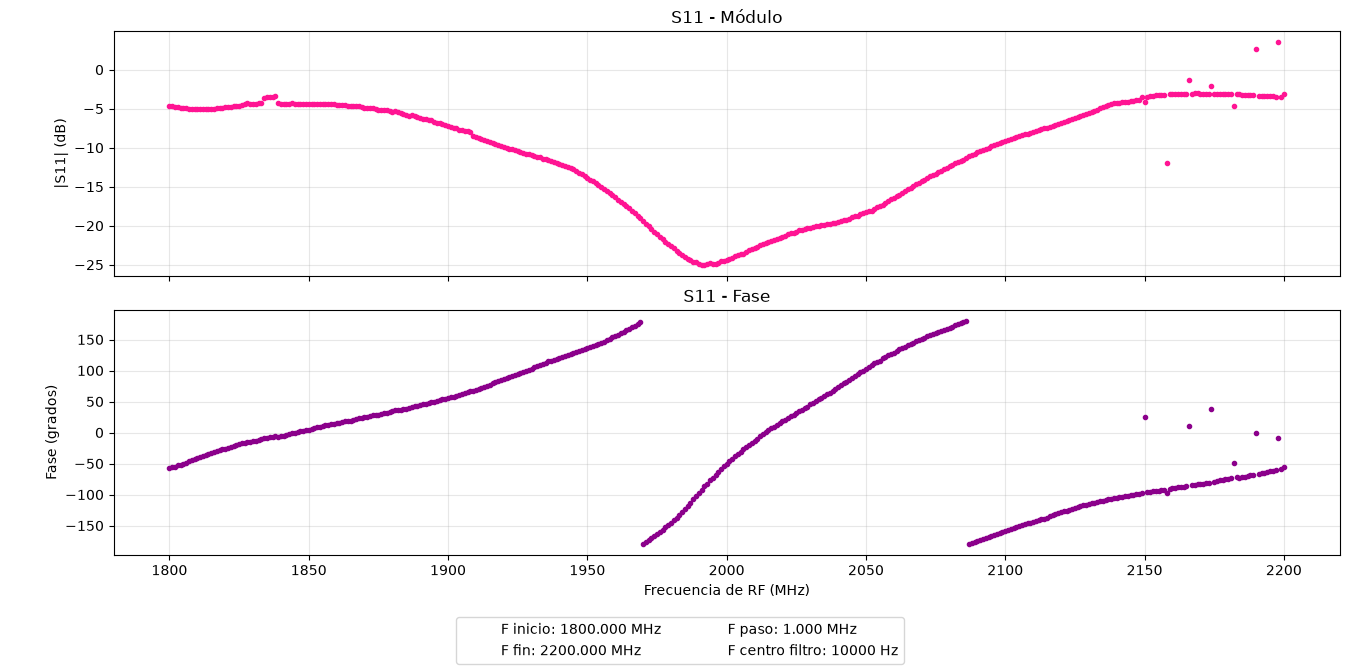
\includegraphics[width=0.7\linewidth]{Imagenes/sensordedorami_15oct_bueno.png}
    \caption{Medición del sensor de glucemia con un dedo.}
    \label{fig:sensorlleno}
\end{figure}


\section{Interfaz de usuario}

Al incluir la interfaz de usuario, se hicieron algunas mediciones para comprobar su funcionamiento, como 50 y 68 $\Omega$ que se pueden ver en las figuras \ref{fig:medinterfaz}. La interfaz agregó el gráfico en un ábaco de Smith.

\begin{figure}[htbp]
    \centering
    % Primera imagen (Página 1) ocupando el 48% del ancho del texto
    \begin{subfigure}[b]{0.48\textwidth}
        \centering
        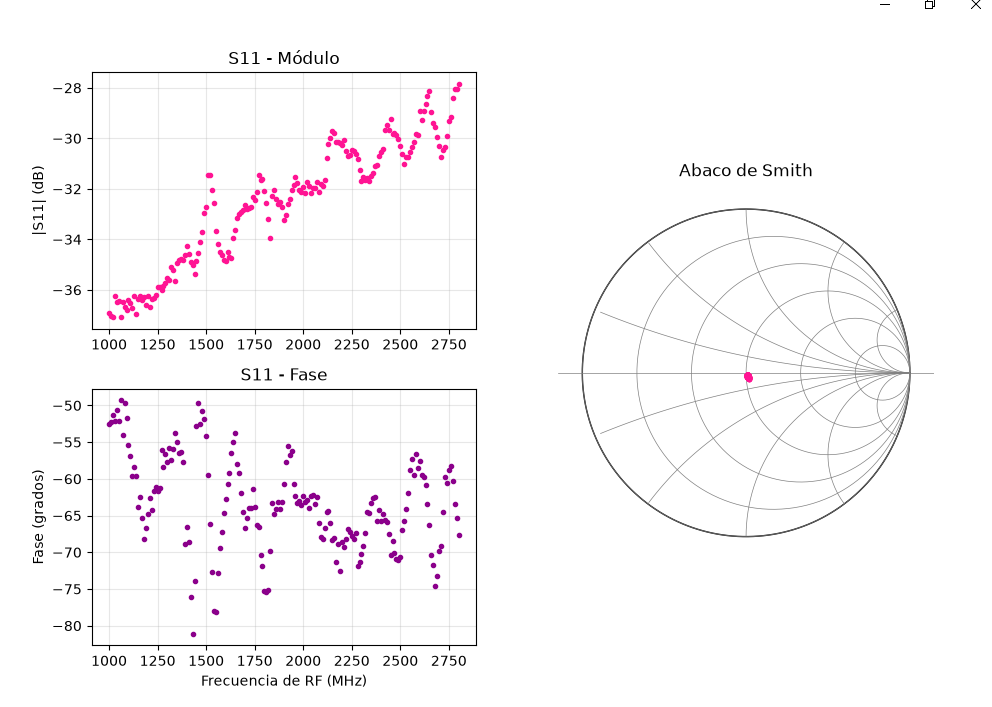
\includegraphics[width=\linewidth]{Imagenes/50R_1000a2800_8oct.png}
        \caption{50 $\Omega$}
        \label{fig:interfaz50}
    \end{subfigure}
    \hfill % Esto agrega un espacio en blanco flexible entre las dos imágenes
    % Segunda imagen (Página 2) ocupando el otro 48%
    \begin{subfigure}[b]{0.48\textwidth}
        \centering
        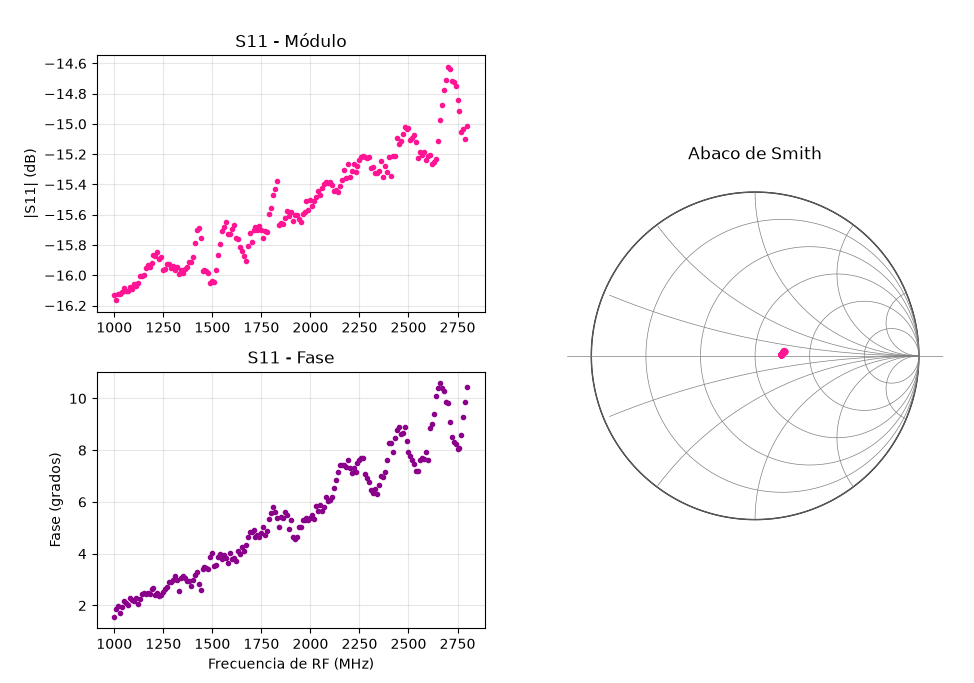
\includegraphics[width=\linewidth]{Imagenes/carga68_8oct_1000a2800.png}
        \caption{68 $\Omega$}
        \label{fig:interfaz68}
    \end{subfigure}
    
    \caption{Mediciones realizadas desde la interfaz de usuario}
    \label{fig:medinterfaz}
\end{figure}